\documentclass{beamer}
\usetheme{Warsaw}
\usecolortheme{beaver}
\hypersetup{pdfstartview={Fit}} % fits the presentation to the window when first displayed
\usepackage{adjustbox} %Used to fit tables to slide

\usepackage{import} % \subimput alows importing of Inkscape pdf+tex files in subfolder

\title[Perception and Working Memory in Neglect]{Perceptual and Working Memory Deficits in Unilateral Neglect} 
\subtitle{}

\author{Jason Locklin}
\institute[University of Waterloo] 
{
  Department of Psychology\\
  University of Waterloo\\
  \bigskip
  Supervisor: Dr. James Danckert
}
\date[August 6, 2015] 
{}% <- QR

\AtBeginSection[]
{
  \begin{frame}
    \frametitle{Experiments}
    \tableofcontents[currentsection]
  \end{frame}
}


\begin{document}

%%%%%%%%%%%%%%%%%%%%%%%% GENERAL INTRODUCTION
\frame{\titlepage}

\section*{}
\begin{frame}
 \frametitle{General Introduction}
 introduction text goes here
\end{frame}



%%%%%%%%%%%%%%%%%%%%%%%% EXPERIMENT ONE

\section[Attention and WM]{Attention and Working Memory in Neglect} 

%%%% COVAT
\subsection*{Covert Orienting}
 \begin{frame}
	 \frametitle{Covert Orienting Task}
  \def\svgwidth{\textwidth}
  \subimport{VWM/}{VWM/fig_COVAT-task.pdf_tex}
 \end{frame}

%%%% VWM
 \subsection*{Visual Working Memory}
  \begin{frame}
	 \frametitle{Visual Working Memory Task}
  \def\svgwidth{\textwidth}
  \subimport{VWM/}{VWM/fig_VWM-task.pdf_tex}
 \end{frame}

 \begin{frame}
	 \frametitle{Response Model Calculations}
 To be added: Slides to explain prob. models based off Fig 2.2.\\
 Need to figure out the best way to explain this fluidly, and also a more thorough
 explenation using appendix slides if necissary.
 \end{frame}

 \begin{frame}
	 \frametitle{Figure 2.3}
	 \centering
	 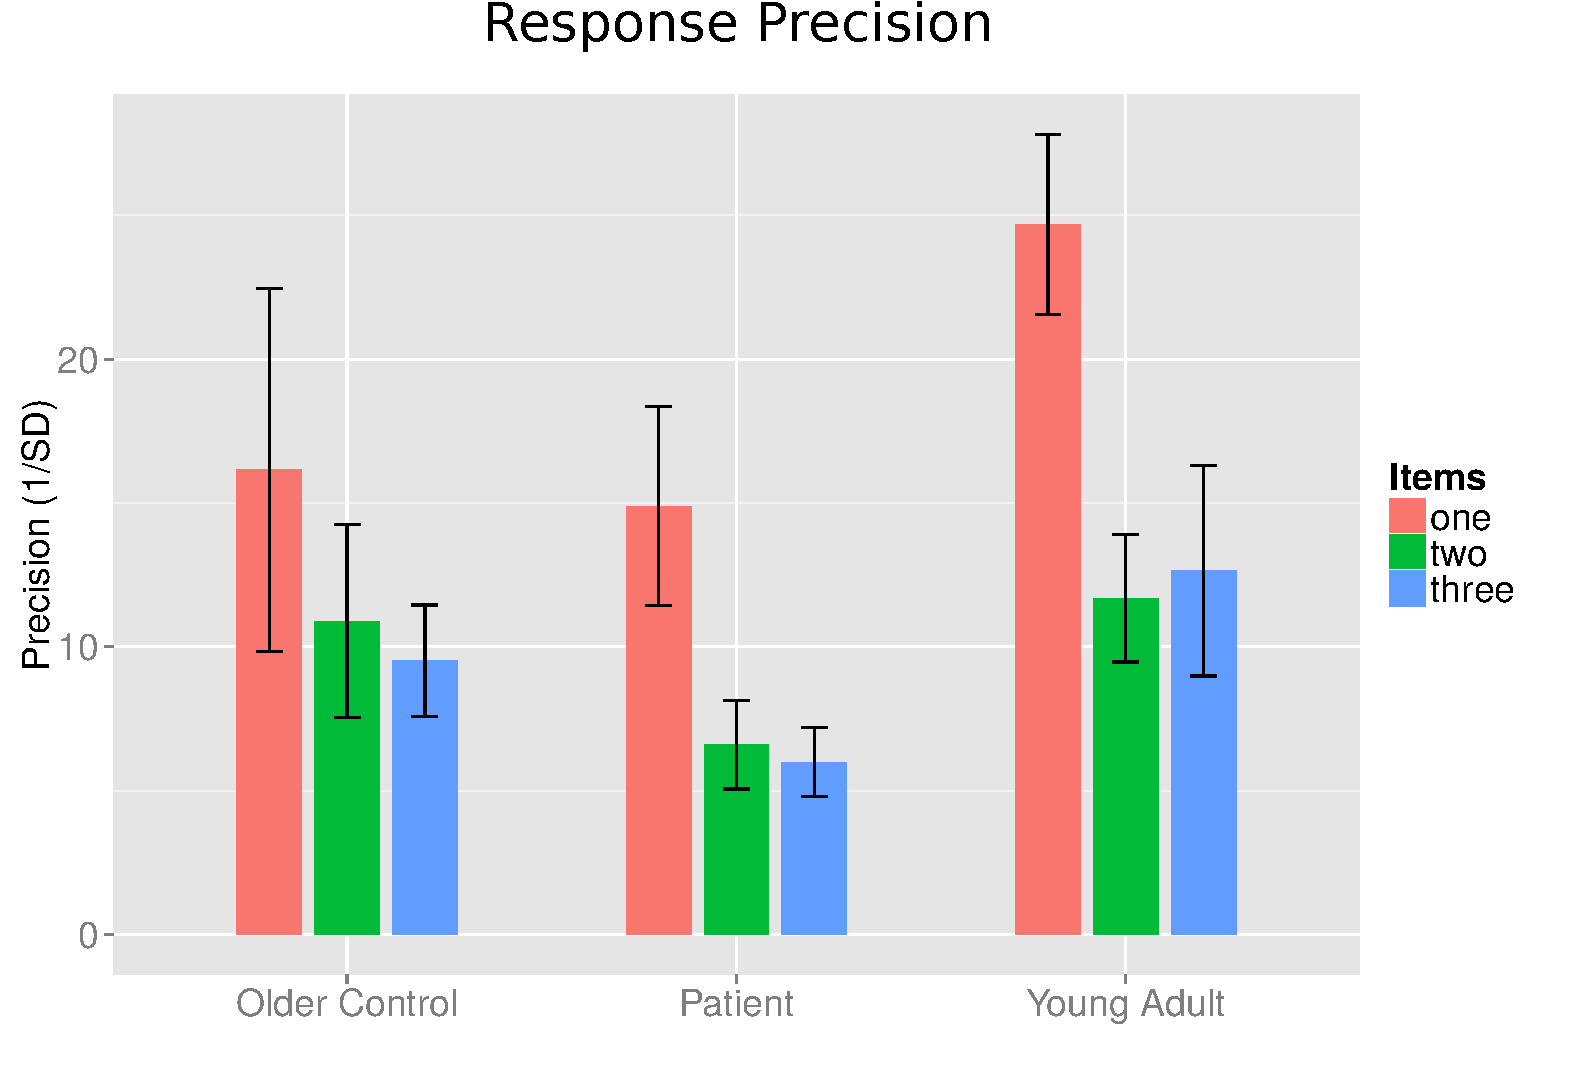
\includegraphics
	 [height=.8\textheight,width=\textwidth,keepaspectratio]
	 {VWM/fig_VWM_Precision.pdf}
 \end{frame}

  \begin{frame}
	 \frametitle{Figure 2.4}
	 \centering
	 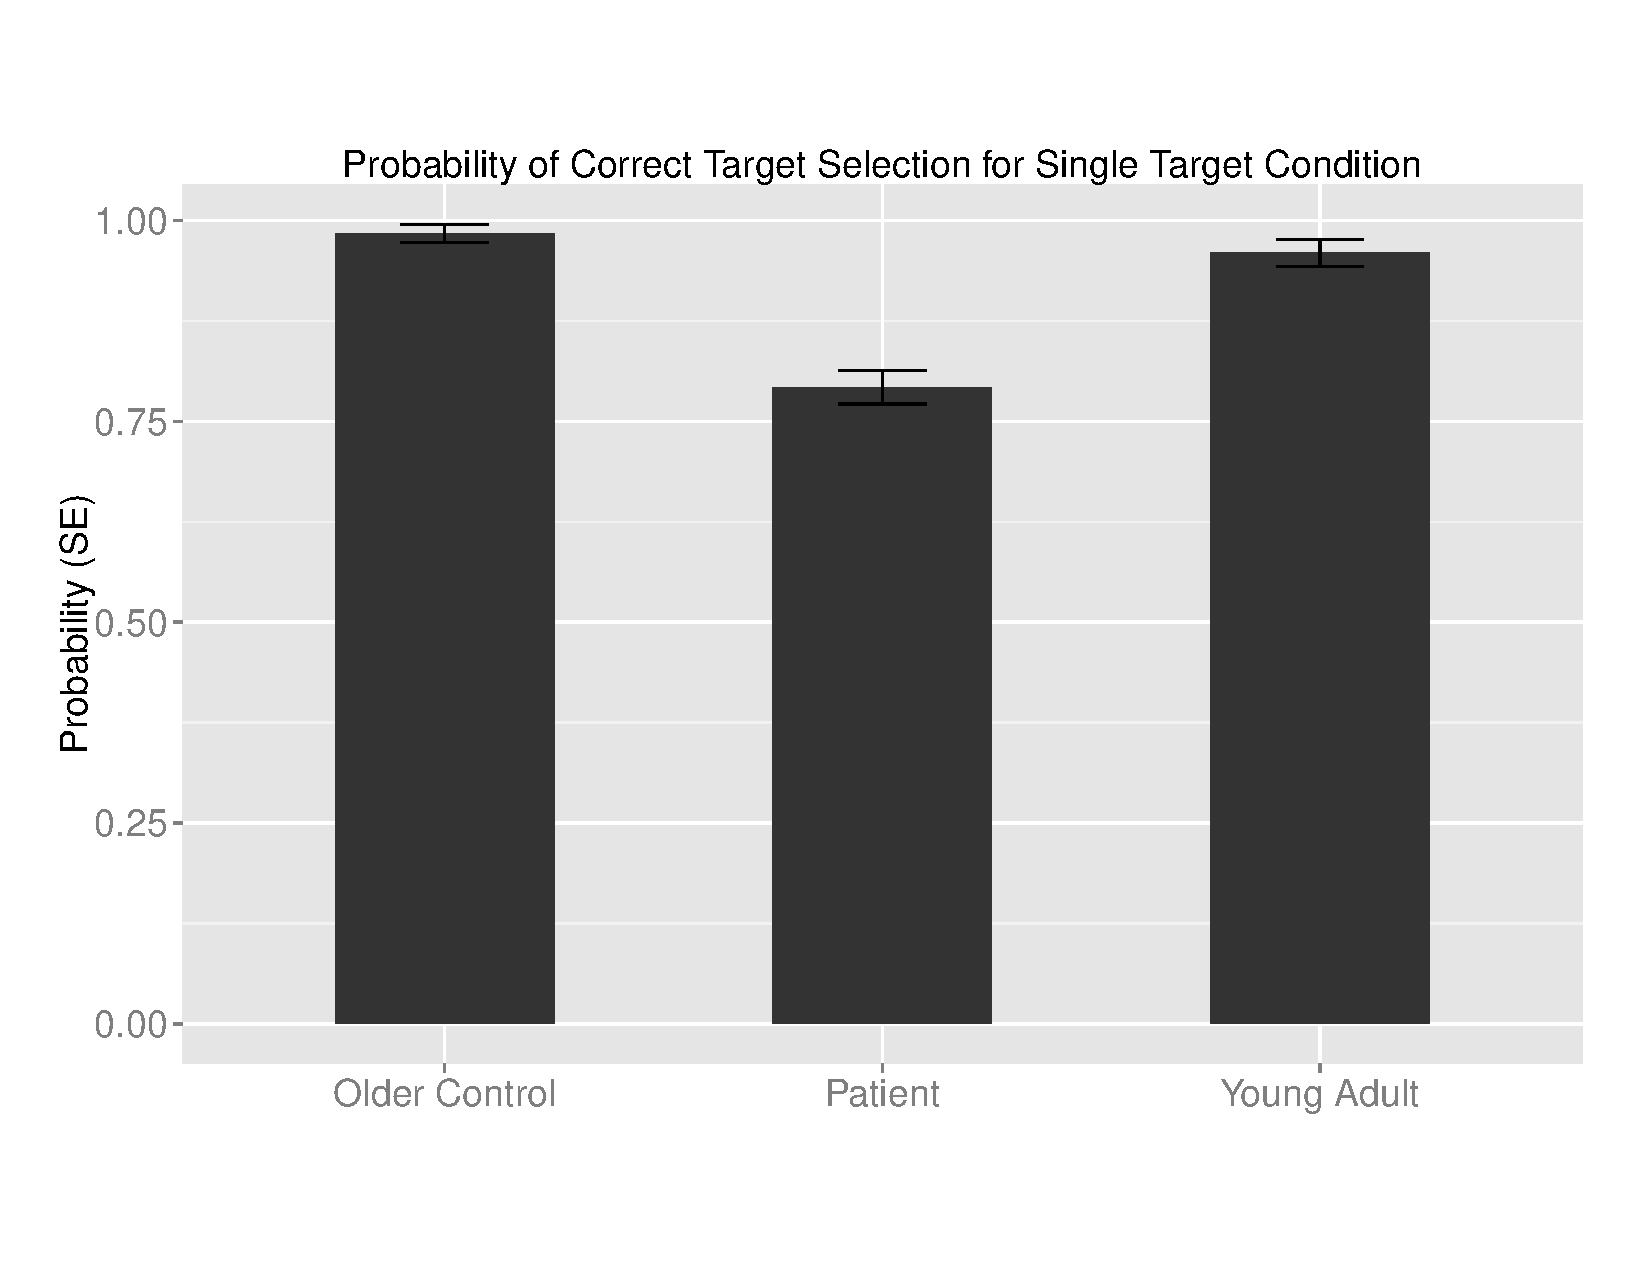
\includegraphics
	 [height=.8\textheight,width=\textwidth,keepaspectratio]
	 {VWM/fig_VWM_1Target.pdf}
 \end{frame}

  \begin{frame}
	 \frametitle{Figure 2.5}
	 \centering
	 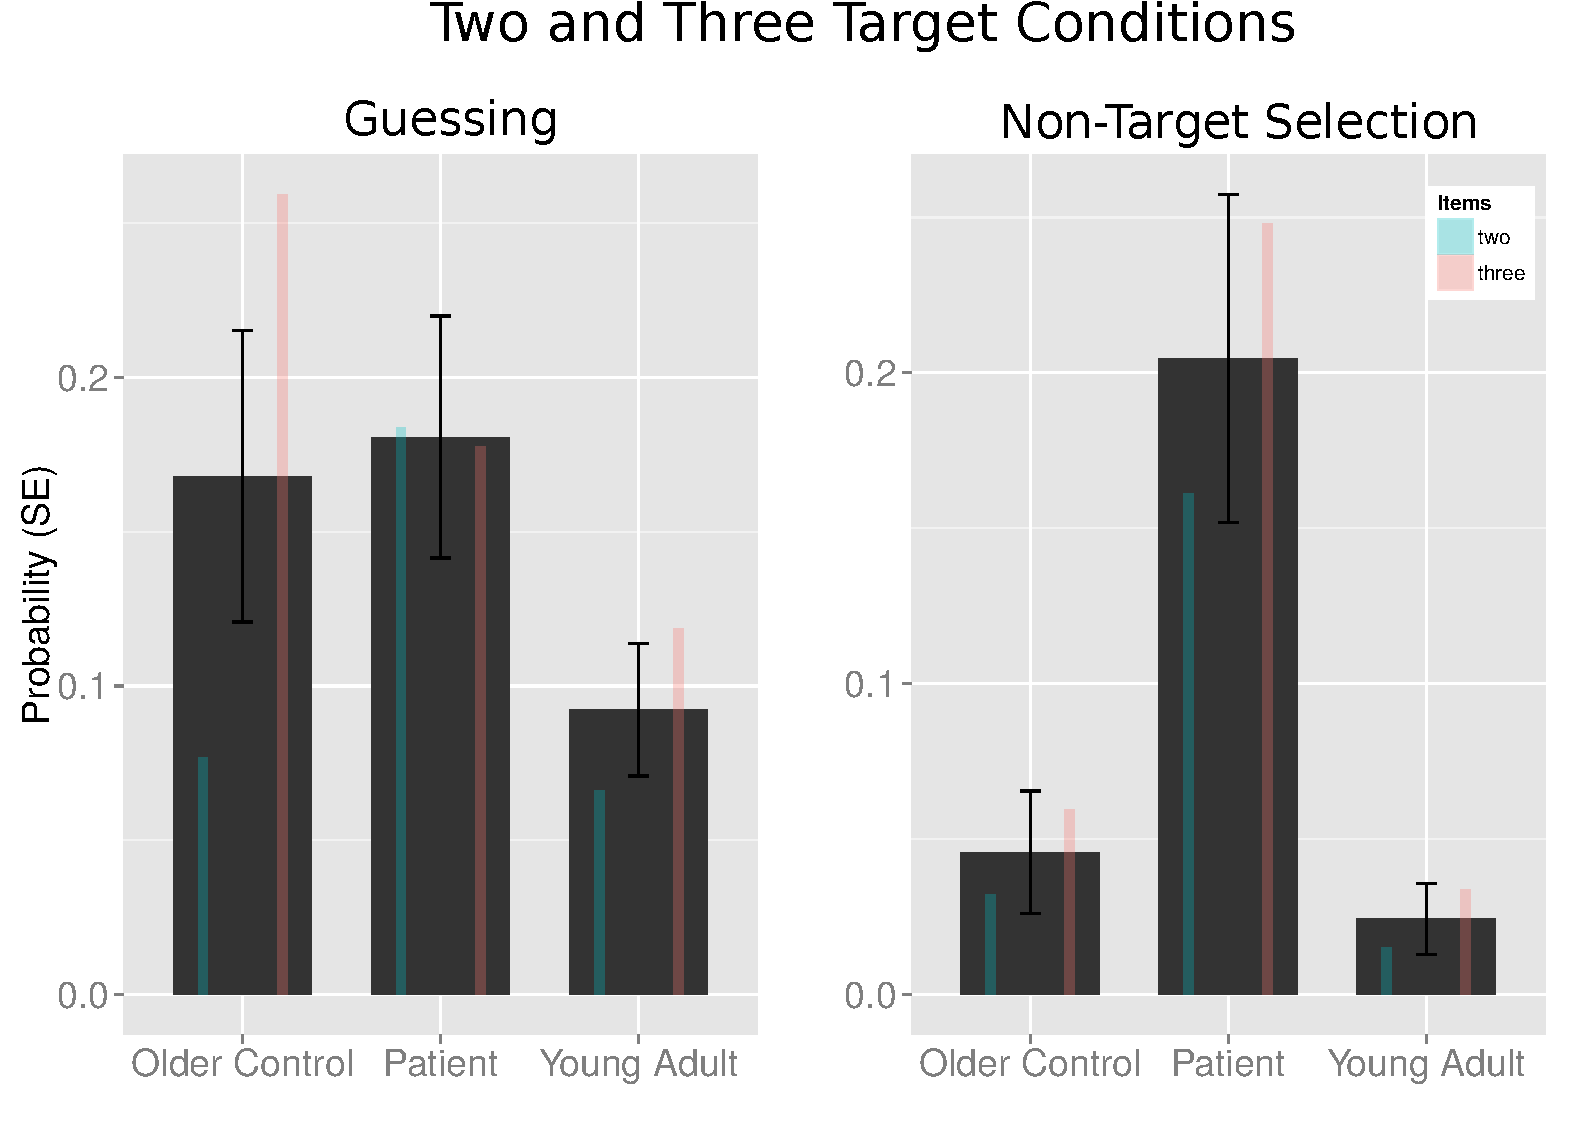
\includegraphics
	 [height=.8\textheight,width=\textwidth,keepaspectratio]
	 {VWM/fig_VWM_MTarget.pdf}
 \end{frame} 
 

%%%%%%%%%%%%%%%%%%%%%%%% EXPERIMENT TWO
 \section[Prisms]{Prism Adaptation and Non-Attention Deficits} 

 \begin{frame}
  \frametitle{This is the first slide}
  text goes here
 \end{frame}

%%%%%%%%%%%%%%%%%%%%%%%% EXPERIMENT THREE
\section[Saccadic Adaptation]{Saccadic Adaptation for Action and Perception} 

 \begin{frame}
  \frametitle{This is the first slide}
  text goes here
 \end{frame}

%%%%%%%%%%%%%%%%%%%%%%%% CONCLUDING MATTER
\section*{}
\begin{frame}
  \frametitle{Conclusions}
  text goes here
 \end{frame}

 \begin{frame}
  \frametitle{Awknowledgements}
  text goes here
 \end{frame}


%%%%%%%%%%%%%%%%%%%%%%%% APPENDIX
\subsection*{Appendix}
\begin{frame}
  \frametitle{Table 2.1}
  \adjustbox{max height=\dimexpr\textheight-5.5cm\relax,
  max width=\textwidth}{
  \begin{tabular}{rrllrrrrlr}
  \hline
 & Age & Sex & Handedness & CES & VWM(1) & VWM(2/3) & Stars & Copying & Bisection \\ 
  \hline
487 &  61 & F & Right & 23.0 & 0.15 & 0.04 & 0& + & 2.2 \\ 
  35 &  51 & F & Right & 27.0 & 0.15 & 0.04 & 17& + & 0.1 \\ 
  489 &  66 & M & Left & 31.0 & 0.25 & 0.08 & 0& + & 1.0 \\ 
  171 &  71 & F & Left & 112.0 & 0.13 & 0.00 & 0& -  & 1.4 \\ 
  454 &  70 & M & Right & 221.5 & 0.23 & 0.17 & 0& + & 6.3 \\ 
  213 &  65 & F & Right & NA & 0.2 & 0.30 & 100& + & 7.3 \\ 
  396 &  85 & M & Right & NA & 0.3 & 0.55 & 87& + & 8.1 \\ 
  465 &  63 & F & Right & NA & 0.3 & 0.45 & 97& + & 12.9 \\ 
   \hline
\end{tabular}
}
 \end{frame}


 
\end{document}
